\documentclass[12pt,xcolor=dvipsnames]{beamer}
\usepackage{amsmath,amssymb,amsfonts}
\usepackage{booktabs}
\usepackage{lmodern}
\usepackage[T1]{fontenc}
\hypersetup{colorlinks,linkcolor=,urlcolor=links}
\usepackage{hyperref}

\usetheme{IS2012Tutorial}
\input{math_definition.tex}

%%%% Other commands to make presentation consistent
\newcommand{\heading}[1]{{\color{red}\textbf{#1}}}
\newcommand{\stress}[1]{{\color{ForestGreen}\textbf{\emph{#1}}}}
\newcommand{\nb}[1]{{\scriptsize \emph{{\color{RoyalPurple}N.B.\ }}\color{Brown}#1}}
% for url to work
\definecolor{links}{HTML}{2A1B81}

%%% For prettier tables
\newlength{\colA}
\newcommand{\aln}[3]{\makebox[#1][#2]{#3}}

% to get references in an easy way, from one BiBTeX file
\usepackage{bibentry}
\def\newblock{\hskip .11em plus .33em minus .07em}
\setbeamertemplate{frametitle continuation}{}

\mode<presentation>

% max figure size is 108 x 72 mm

\author{Florian Metze, Samuel Thomas, \\
  Bhuvana Ramabhadran, and Brian Kingsbury}
\title{{\color{Maroon} Pushing the frontiers of speech processing --- What does it take to tackle new languages and domains?}}
\institute{Carnegie Mellon University and IBM}
\date{\today}

\sloppy

\begin{document}

\section{Title}

\begin{frame}
  \titlepage
\end{frame}

\begin{frame}
  \frametitle{Florian Metze}
  \begin{columns}[T]
    \column{2in}
    \begin{itemize}
    \item Associate Research Professor at Carnegie Mellon University (LTI/SCS)
    \item End-to-end Speech Recognition
    \item Articulatory Features for Speech Recognition
    \item Multi-media Analysis
    \item \texttt{fmetze@cs.cmu.edu}
    \end{itemize}
    \column{2in}
    \framebox{\includegraphics[width=2in]{figures/Florian}}
  \end{columns}
\end{frame}

\begin{frame}
  \frametitle{Samuel Thomas}
  \begin{columns}[T]
    \column{2in}
    \begin{itemize}
    \item 
    \item \texttt{sthomas@us.ibm.com}
    \end{itemize}
    \column{2in}
    % \framebox{\includegraphics[width=2in]{Sam}}
  \end{columns}
\end{frame}

\begin{frame}
  \frametitle{Bhuvana Ramabhadran}
  \begin{columns}[T]
    \column{2in}
    \begin{itemize}
    \item 
    \item \texttt{bhuvana@us.ibm.com}
    \end{itemize}
    \column{2in}
    % \framebox{\includegraphics[width=2in]{Bhuvana}}
  \end{columns}
\end{frame}

\begin{frame}
  \frametitle{Brian Kingsbury}
  \begin{columns}[T]
    \column{2in}
    \begin{itemize}
    \item Research Scientist in the IBM Watson Group
    \item Deep Learning
    \item Automatic Speech Recognition
    \item Keyword Search
    \item \texttt{bedk@us.ibm.com}
    \end{itemize}
    \column{2in}
    \framebox{\includegraphics[width=2in]{figures/Brian}}
  \end{columns}
\end{frame}


\begin{frame}
  \frametitle{Outline (3 hours)}
  \begin{enumerate}
  \item Introduction
  \item Tackling a New Language
  \item Tackling a New Domain
  \item Lessons Learnt with Current Neural Network Technologies
  \item Research Topics, Challenges, and New Ideas
  \item End-to-End Systems
  \item Virtual Machines and Tools
  \item Conclusions
  \end{enumerate}
\end{frame}

\begin{frame}
  \begin{center}
    {\color{Maroon}\Huge Introduction}
  \end{center}
\end{frame}

%% put section outline here
\begin{frame}{Introduction}{Outline}
  \begin{enumerate}
  \item The shift in speech based user interfaces
  \item Building applications on the information rich speech signal
    \begin{itemize}
    \item Automatic speech recognition
    \item Speaker recognition
    \item Speaker diarization
    \item Language identification
    \item Processing social signals
    \end{itemize}
  \item Impact of speech technologies across languages and domains
  \item The Speech Recognition Case Study
    \begin{itemize}
    \item What is under the hood for speech recognition technologies?
    \item Building various ASR module and the impact of trascribed data
    \end{itemize}
  \item Building ASR Systems in New Languages
    \begin{itemize}
    \item Building from ASR systems from scratch
    \item Is there room for sharing data from other languages?
    \end{itemize}
  \item Building ASR Systems in New Domain
    \begin{itemize}
    \item Adaptation of an existing ASR system
    \end{itemize}
  \end{enumerate}
\end{frame}


\begin{frame}
  \begin{center}
    {\color{Maroon}\Huge Tackling New Languages}
  \end{center}
\end{frame}

\begin{frame}{Tackling New Languages}{Outline}
  \begin{enumerate}
  \item IARPA Babel
  \item Audio Keyword Search
  \item What Language Characteristics Matter?
  \item A Recipe for a New Language
    \begin{itemize}
    \item Pronunciations
    \item Flat-start Initialization
    \item Multilingual Features
    \item Web Text
    \end{itemize}
  \end{enumerate}
\end{frame}

\begin{frame}{The IARPA Babel Program}{}
  \Large{``\ldots to \alert{rapidly develop} speech recognition
    capability for keyword search in a previously unstudied
    language, working with speech recorded in a variety of
    conditions with limited amounts of transcription.''}\par
\end{frame}

\begin{frame}{Rapid Development}{Time allowed for surprise language model building}
  \centering
  \begin{tabular}{@{}cl@{}} \toprule
    {\bf Period} & \multicolumn{1}{c}{\bf Time} \\ \midrule
    1 & 4 weeks \\
    2 & 3 weeks \\
    3 & 2 weeks \\
    4 & 1 week  \\ \bottomrule
  \end{tabular}
\end{frame}

\begin{frame}{The IARPA Babel Program}{}
  \Large{``\ldots to rapidly develop speech recognition
    capability for keyword search in a \alert{previously unstudied
      language}, working with speech recorded in a variety of
    conditions with limited amounts of transcription.''}\par
\end{frame}

\begin{frame}{Babel Languages}{}
  \begin{center}
  \begin{tabular}{@{}llll@{}} \toprule
    \multicolumn{1}{c}{\bf Period 1} & \multicolumn{1}{c}{\bf Period 2} & \multicolumn{1}{c}{\bf Period 3} & \multicolumn{1}{c}{\bf Period 4} \\ \midrule
    Cantonese  & Assamese       & Kurmanji Kurdish & Pashto \\
    Pashto     & Bengali        & Tok Pisin        & Guaran\'{i} \\
    Turkish    & Haitian Creole & Cebuano          & Igbo \\
    Tagalog    & Lao            & Kazakh           & Amharic \\
    Vietnamese & Zulu           & Telugu           & Mongolian \\
               & Tamil          & Lithuanian       & Javanese \\
               &                & Swahili          & Dholuo \\
               &                &                  & Georgian \\ \bottomrule
  \end{tabular}
  \end{center}
  \vfill
  \nb{These will be available from the LDC at \$US 25.00 per language for non-members.}
\end{frame}

\begin{frame}{The IARPA Babel Program}{}
  \Large{``\ldots to rapidly develop speech recognition
    capability for keyword search in a previously unstudied
    language, working with speech recorded in a variety of
    conditions with \alert{limited amounts of transcription}.''}\par
\end{frame}

\begin{frame}{Limited resources}{Hours of transcribed training data}
  \settowidth{\colA}{100}
  \begin{center}
    \begin{tabular}{@{}cc@{}} \toprule
      {\bf Period} & {\bf Hours} \\ \midrule
      1 & 100 \\
      2 & \aln{\colA}{r}{10} \\
      3 & \aln{\colA}{r}{3}  \\
      4 & \aln{\colA}{r}{40} \\ \bottomrule
    \end{tabular}
  \end{center}
  \vfill
  \nb{In Periods 3 and 4, no phonetic lexicons.}
\end{frame}

\begin{frame}{The IARPA Babel Program}{}
  \Large{``\ldots to rapidly develop speech recognition
    capability for \alert{keyword search} in a previously unstudied
    language, working with speech recorded in a variety of
    conditions with limited amounts of transcription.''}\par
\end{frame}

\begin{frame}{What is keyword search, and why focus on it?}{}
  {\bf Detection task}: given
    \begin{itemize}
    \item a word or short phrase and
    \item a collection of speech data,
    \end{itemize}
    does it occur, and if so where does it occur, and how confident are you?
    \vfill
    We can build practical keyword search from
    \alert{unreliable} speech recognition.
\end{frame}

\begin{frame}{Weighted Finite-State Acceptors}{}
  A \alert{weighted finite-state acceptor} compactly represents a set
  of strings, with a score assigned to each string.
  \vfill
  Formally, a WFSA comprises
  \begin{description}
  \item[states] some of which are start states, end states, or both;
    and
  \item[edges] between states, labeled with symbols from a finite
    alphabet and scores.
  \end{description}
\end{frame}

\begin{frame}{An Example}{}
  \begin{center}
    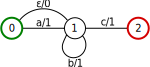
\includegraphics[width=72mm]{figures/WFSA}
  \end{center}
  \vfill
  Represents {\tt a?b*c} and the score of each string is its length.
\end{frame}

\begin{frame}{Weighted Finite-State Transducers}{}
  A \alert{weighted finite-state transducer} compactly represents a
  relation between two sets of strings, with a score assigned to each
  output string.
  \vfill
  Formally, a WFST comprises
  \begin{description}
  \item[states] some of which are start states, end states, or both;
    and
  \item[edges] between states, labeled with input symbols from a
    finite alphabet, output samples from a (potentially different)
    finite alphabet, and scores.
  \end{description}
\end{frame}

\begin{frame}{An Example}{}
  \begin{center}
    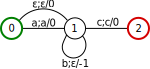
\includegraphics[width=72mm]{figures/WFST}
  \end{center}
  \vfill
  Maps strings in {\tt a?b*c} to {\tt a?c} by deleting {\tt b} symbols
  and the score of each string the change in its length.
\end{frame}

\begin{frame}{Composition}{}
  \begin{center}
    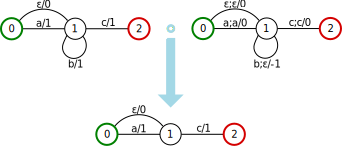
\includegraphics[width=96mm]{figures/Composition}
  \end{center}
  \vfill
  Given WFSA $\mathcal{S}$ and WFST $\mathcal{T}$, their composition
  $\mathcal{T} \circ \mathcal{S}$ is a WFSA that represents the set of
  strings (and corresponding scores) obtained by applying
  $\mathcal{T}$ to the set of strings represented by $\mathcal{S}$.
\end{frame}

\begin{frame}{Roadmap for WFST-based keyword search}{}
  \begin{enumerate}
  \item Form a WFST index representing a relation between
    \begin{description}
      \item[inputs] all high-probability strings of words or phones in
        the collection,
      \item[outputs] times of occurrence of the words or phones, and
      \item[scores] probabilities of the strings;
    \end{description}
    \item Form a WFSA representing a query; then
    \item \alert{compose} the query WFSA with the index WFST to
      perform the search.
  \end{enumerate}
\end{frame}

%% WFST search:  index generation (token and phonetic)
\begin{frame}{Building an index}{1. Generate a lattice for each segment in the collection.}
  \begin{center}
    
\includegraphics[width=36mm]{figures/lattice}
  \end{center}
  \begin{overlayarea}{\textwidth}{24mm}
    \begin{columns}[t]
      \column{54mm}
      \onslide<1>{
        \centerline{\bf Lattice}
        \begin{description}
        \item[Nodes] times
        \item[Edges] words (or phones) and posterior probabilities
        \end{description}
      }
      \column{54mm}
      \onslide<2>{
        \centerline{\bf Transducer}
        \begin{description}
        \item[Inputs] words (or phones)
        \item[Outputs] times
        \item[Scores] negative log-posteriors
        \end{description}
      }
    \end{columns}
  \end{overlayarea}
\end{frame}

\begin{frame}{Building an index}{2. Produce the factor automaton for each segment.}
  \begin{center}
    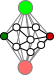
\includegraphics[width=36mm]{figures/factor}
    \end{center}
  \vfill
  Added edges have $\epsilon$ inputs, $\epsilon$ outputs, and no costs.
\end{frame}

\begin{frame}{Building an index}{3. Connect all the factor automata in parallel.}
  \begin{center}
    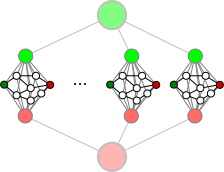
\includegraphics[width=66mm]{figures/index}
    \end{center}
  \vfill
  Added edges from start have $\epsilon$ inputs, segment ID outputs, and no costs.
  Added edges to end have $\epsilon$ inputs, $\epsilon$ outputs, and no costs.
\end{frame}

\begin{frame}{Building a query}{}
  In-vocabulary queries are simple:
  \begin{enumerate}
  \item use a word-based WFST index, and
  \item represent queries as word-level linear-chain WFSAs.
  \end{enumerate}
  \vfill
  Queries containing \alert{out-of-vocabulary} words are more challenging.
\end{frame}

\begin{frame}{Handling out-of-vocabulary queries}{}
  \begin{enumerate}
  \item represent queries as phone-level linear-chain WFSAs,
  \item compose the WFSAs with a WFST \alert{confusability} model,
  \item prune the resulting WFSAs, and
  \item {\bf if a word-based index is used}, compose the query WFSAs
    with a WFST that maps phone sequences back to words.
  \end{enumerate}
  \vfill
  The confusability model is created by running speech recognition on
  the training data and counting co-occurrences of reference and
  hypothesized phones.
  \vfill
  \nb{This is a form of query expansion, which is well
    studied in the information retrieval literature.}
\end{frame}

\begin{frame}{How do we measure keyword search performance?}
  {Actual Term-Weighted Value (ATWV)}
  \begin{equation*}
    \text{ATWV}(\theta) = \frac{1}{N}\sum_{q}
    \left[
      \frac{N_{\text{hit}}(q;\theta)}{N_{\text{true}}(q)} -
      \beta \frac{N_{\text{FA}}(q;\theta)}{T - N_{\text{true}}(q)}
      \right]
  \end{equation*}
  \begin{itemize}
  \item There are $N$ test queries indexed by $q$,
  \item $\theta$ is a decision threshold,
  \item $N_{\text{hit}}(q;\theta)$ is the number of correct detections and
  \item $N_{\text{FA}}(q;\theta)$ is the number of false alarms for
    query $q$ at decision threshold $\theta$, 
  \item $N_{\text{true}}(q)$ is the number of occurrences of query $q$
    in the test audio,
  \item $T$ is the duration of the test audio in seconds, and
  \item $\beta = 999.9$ is a weight on the penalty for false alarms.
  \end{itemize}
\end{frame}

\begin{frame}{Breaking it down}{}
  \begin{overlayarea}{\textwidth}{56mm}
  \only<1>{
  \begin{equation*}
    \text{ATWV}(\theta) = \frac{1}{N}\sum_{q}
    \left[
      {\color{red}\frac{N_{\text{hit}}(q;\theta)}{N_{\text{true}}(q)}} -
      \beta \frac{N_{\text{FA}}(q;\theta)}{T - N_{\text{true}}(q)}
      \right]
  \end{equation*}
  }
  \only<2>{
  \begin{equation*}
    \text{ATWV}(\theta) = \frac{1}{N}\sum_{q}
    \left[
      \frac{N_{\text{hit}}(q;\theta)}{N_{\text{true}}(q)} -
      {\color{red}\beta \frac{N_{\text{FA}}(q;\theta)}{T - N_{\text{true}}(q)}}
      \right]
  \end{equation*}
  }
  \only<3>{
  \begin{equation*}
    \text{ATWV}(\theta) = \frac{1}{N}\sum_{q}
    \left[
      \frac{N_{\text{hit}}(q;\theta)}{N_{\text{true}}(q)} -
      \beta \frac{N_{\text{FA}}(q;\theta)}{T - N_{\text{true}}(q)}
      \right]
  \end{equation*}
  }
  \vspace*{8mm}
  \begin{itemize}
  \item<1-> Hits earn a reward of $\frac{1}{N \cdot N_{\text{true}}(q)}$, so
    rare terms are more valuable.
  \item<2-> False alarms incur a constant loss of approximately
    $\frac{\beta}{N \cdot T}$ (because $T \gg N_{\text{true}}(q)$ for all $q$).
  \item<3-> Perfect performance scores $\text{ATWV} = 1.0$, while
    empty output scores $\text{ATWV} = 0.0$.  $\text{ATWV} < 0.0$
    means you have too many false alarms!
  \end{itemize}
  \end{overlayarea}
  \vfill
  \nb{Score normalization is important under the ATWV metric.  For
    more details on this issue, please see \cite{Wang2014}.}
\end{frame}

\begin{frame}{Babel Languages}{}
  \begin{center}
    \begin{tabular}{@{}llll@{}} \toprule
      \multicolumn{1}{c}{\bf Period 1} & \multicolumn{1}{c}{\bf Period 2} & \multicolumn{1}{c}{\bf Period 3} & \multicolumn{1}{c}{\bf Period 4} \\ \midrule
      Cantonese  & Assamese       & Kurmanji Kurdish & Pashto \\
      Pashto     & Bengali        & Tok Pisin        & Guaran\'{i} \\
      Turkish    & Haitian Creole & Cebuano          & Igbo \\
      Tagalog    & Lao            & Kazakh           & Amharic \\
      Vietnamese & Zulu           & Telugu           & Mongolian \\
                 & Tamil          & Lithuanian       & Javanese \\
                 &                & Swahili          & Dholuo \\
                 &                &                  & Georgian \\ \bottomrule
    \end{tabular}
  \end{center}
\end{frame}

\begin{frame}{What language characteristics matter?}{}
  \begin{enumerate}
  \item Morphology
  \item Writing system
  \item Tonal languages
  \item Amount of available training data
  \end{enumerate}
\end{frame}

%% Morphology and vocabulary growth
\begin{frame}{Morphology}{}
  The morphology of a language refers to the structure of its words.
  Specifically, are words atomic, or are they composed from meaningful
  parts?
  \vfill
  {\color{DarkerBlue}\bf English example} \\
  re+ +do+ +er --- one who is performing some action again
  \vfill
  Languages with \alert{agglutinative} morphology have large
  inventories of words formed by the composition of smaller units
  (morphs).
  \vfill
  One way to characterize this is through vocabulary growth.
\end{frame}

\begin{frame}{Vocabulary Growth for Babel Languages}{}
  \begin{center}
    \includegraphics[width=108mm]{figures/vocGrowth}
  \end{center}
\end{frame}

\begin{frame}{Mitigating Rapid Vocabulary Growth}{}
  Out-of-vocabulary words are more likely to occur in test data for
  languages with rapid vocabulary growth, which will degrade speech
  recognition and keyword search performance.
  \vfill
  Two ways to reduce the impact:
  \begin{description}[morph models]
    \item[morph models] base the vocabulary on morphs instead of
      words, and
    \item[web text] expand the vocabulary by collecting text from the
      web.
  \end{description}
\end{frame}

\begin{frame}{Morph Models}{}
  Recipe:
  \begin{enumerate}
  \item Segment the training text into morph-like units using
    Morfessor~\cite{Morfessor} or some other tool.
  \item Generate a pronunciation lexicon for the morphs.
  \item Train a language model on the segmented training text.
  \end{enumerate}
  \vfill
  Task-specific considerations:
  \begin{description}
  \item[ASR]
    \begin{itemize}
    \item Recomposing morphs into words is challenging.
    \end{itemize}
  \item[KWS]
    \begin{itemize}
      \item Need to decompose queries into morphs.
      \item Best results obtained by doing word and morph search, and
        fusing the results.
    \end{itemize}
  \end{description}
\end{frame}

\begin{frame}{Keyword Search Results with Morph Models}{}
  \begin{columns}[c]
    \column{68mm}
    \centering
    \begin{tabular}{@{}lcc@{}} \toprule
      & {\bf Word} & {\bf Word+Morph} \\
      {\bf Language} & {\bf MTWV} & {\bf MTWV} \\ \midrule
      Zulu     & 0.1817 & 0.2305 \\
      Assamese & 0.2643 & 0.2797 \\ \bottomrule
    \end{tabular}
    \column{40mm}
    \centering{\includegraphics[width=40mm]{figures/vocGrowthThumb}}
  \end{columns}
  \vfill
  \nb{Maximum Term-Weighted Value (MTWV) is ATWV with an oracle
    decision threshold.}
\end{frame}

\begin{frame}{Web Text}{}
  General considerations:
  \begin{itemize}
  \item How much web presence does the language have?
    \begin{itemize}
    \item Swahili: plenty
    \item Dholuo: sparse
    \end{itemize}
  \item How easy is it to generate queries returning the target language?
    \begin{itemize}
    \item Amharic has its own Unicode range, so it is easy.
    \item Tagalog contains many English and Spanish loanwords, so it
      is difficult.
    \end{itemize}
  \item Normalization is a must!
  \end{itemize}
\end{frame}

\begin{frame}{Web Text}{}
  Task-specific considerations:
  \begin{description}
  \item[ASR] Improvements may be small due to genre mismatch (LM is important).
  \item[KWS] Better vocabulary coverage improves performance (LM is not important).
  \end{description}
\end{frame}

\begin{frame}{Impact of Web Text}{}
  \centering
  \begin{tabular}{@{}lcd{5.1}d{3.1}cc@{}} \toprule
    & & \multicolumn{1}{c}{\bf Train} & \multicolumn{1}{c}{\bf Voc.} &               &            \\
    {\bf Language} & {\bf Web?} & \multicolumn{1}{c}{\bf size} & \multicolumn{1}{c}{\bf size} & {\bf \% WER} & {\bf MTWV} \\ \midrule


    Igbo        & N &    45.3 & 16.5 & 66.5 & 0.2387 \\
                & Y &   707.  & 19.3 & 66.5 & 0.2389 \\ \midrule
    Guaran\'{i} & N &    46.8 & 26.3 & 53.5 & 0.4562 \\
                & Y &   437.  & 36.8 & 53.5 & 0.4665 \\ \midrule
    Mongolian   & N &    51.2 & 23.6 & 61.1 & 0.3497 \\
                & Y & 55300.  & 217. & 60.4 & 0.3849 \\ \bottomrule
  \end{tabular}
  \vfill
  \raggedright
  Word counts are in thousands.
\end{frame}

%% \begin{frame}{Impact of Web Text}{}
%%   \centering
%%   \begin{tabular}{@{}lcd{3.1}d{2.1}cc@{}} \toprule
%%     & & \multicolumn{1}{c}{\bf Voc.}     & \multicolumn{1}{c}{\bf \% OOV}  &              &            \\
%%     {\bf Language} & {\bf Web?} & \multicolumn{1}{c}{\bf size (K)} & \multicolumn{1}{c}{\bf queries} & {\bf \% WER} & {\bf MTWV} \\ \midrule
%%     Igbo        & N & 16.5 & 11.9 & 66.5 & 0.2387 \\
%%                 & Y & 19.3 & 11.6 & 66.5 & 0.2389 \\ \midrule
%%     Guaran\'{i} & N & 26.3 & 13.8 & 53.5 & 0.4562 \\
%%                 & Y & 36.8 & 12.9 & 53.5 & 0.4665 \\ \midrule
%%     Mongolian   & N & 23.6 & 12.2 & 61.1 & 0.3497 \\
%%                 & Y & 217. &  3.8 & 60.4 & 0.3849 \\ \bottomrule
%%   \end{tabular}
%% \end{frame}

%% Writing system ... only matters if you don't have a phonetic
%% pronunciation lexicon
%% - Ideographic
%% - Alphabet
%% - Abjad
%% - Abugida
%% Ideographic languages require a character-to-pronunciation
%% lexicon, while in many cases the other writing systems may be
%% handled with simple rule-based spelling-to-sound conversion.

%% Tonal languages
%% If so, must represent pitch
%% explicit - e.g. FFV features
%% implicit - e.g. high-resolution Mel spectral features in NN
%% give results for Lao

%% Amount of available training data
%%   multilingual feature front-ends
%%   multilingual AMs
%%   Data augmentation
%%   Semi-supervised training

%% A Recipe for a New Language (do a VLLP and a recent FLP?)
%% Pronunciations
%% Flat-start Initialization
%% Multilingual Features
%% Web Text

%% \begin{frame}{}{}
%% \end{frame}


\begin{frame}
  \begin{center}
    {\color{Maroon}\Huge Tackling a New Domain}
  \end{center}
\end{frame}

%% put section outline here


\section{Research Topics, Challenges, and New Ideas}

% bedk - \par at end ensures proper line spacing
\begin{frame}
  \begin{center}
    {\color{Maroon}\Huge Research Directions and New Modeling Techniques\par}
  \end{center}
\end{frame}

%%%% ----------------------------
%%%%     CHALLENGES
%%%% ----------------------------

\begin{frame}
  \begin{center}
    {\color{Maroon}\Huge Challenges}
  \end{center}
\end{frame}

\begin{frame}{Are we there yet?}
  \begin{center}
    \includegraphics[height=65mm]{figures/ASR9}
  \end{center}
\end{frame}

\begin{frame}{Is that it?}
  \begin{center}
    \includegraphics[height=65mm]{figures/am-mlp}
  \end{center}
\end{frame}

\begin{frame}{Challenges}
  \begin{itemize}
  \item What could be wrong?
  \item We are using a solid statistical framework
  \item We know how to extract ``features''
  \item We know how to learn models
  \item We know how to search for the best path
  \item So we must be doing the right thing!
  \end{itemize}
\end{frame}

\begin{frame}{Really? Let's think about this some more!}
  \begin{itemize}
    \item Given: an observation (ADC, FFT, ...)\\
      $\boldsymbol{X} = \boldsymbol{x}_1, \boldsymbol{x}_2, ..., \boldsymbol{x}_T$
    \item Wanted: the corresponding word sequence\\
      $W = w_1, w_2, ..., w_m$
    \item Search for the most likely word sequence $W'$
    \item Fundamental Equation of ASR: \\
      $W' = \arg \max_W P(W|\boldsymbol{X}) = \arg \max p(\boldsymbol{X}|W) P(W) $ \hspace{1cm} (Bayes)
    \item $p(\boldsymbol{X}|W)$ is the ``acoustic model''
    \item $P(W)$ is the ``language model''
    \item And how are we evaluating this?
  \end{itemize}
\end{frame}

\begin{frame}{Word Error Rate}
  \begin{itemize}
    \item \#errors / \#words (in reference)
    \item (\#insertions + \#substitutions + \#deletions) / \#words
    \item Example:\\
      \begin{tabular}{lccccc}
        Reference  &            & \texttt{SHOW} & \texttt{ME} & \texttt{THE} & \texttt{INTERFACE} \\
        Hypothesis & \texttt{I} & \texttt{SHOW} & \texttt{ME} &              & \texttt{FACE} \\
        Alignment  & \textsc{I} &               &             & \textsc{D}   & \textsc{S} \\
      \end{tabular}
    \item WER=$3/4=75\%$
    \item So? Did anyone see this in the fundamental equation? $P(W|\boldsymbol{X})$, anyone?
  \end{itemize}
\end{frame}

\begin{frame}{Fundamentals revisited}
  \begin{itemize}
  \item If we are optimizing for $P(W|\boldsymbol{X})$,
    we are optimizing for the \textit{sentence} error rate, $\langle P(W|\boldsymbol{X}) \rangle$
  \item But we want $P(\langle w_i \rangle|\boldsymbol{X})$ for $W=w_1,w_2, ..., w_m$ (for one sentence)
  \item Clearly, this is not the same thing!
  \item However, in practice, it is not complete uncorrelated either
    \begin{itemize}
    \item[$\rightarrow$] And there are ways to deal with this (confusion networks, discriminative training)
    \end{itemize}
  \item Similarly, for spoken term detection, dialog systems, etc.
  \end{itemize}
\end{frame}

\begin{frame}{The speech recogition conundrum}
  \begin{itemize}
  \item We want to optimize word error rate (or whatever)\\
    \vspace{1cm}
  \item We optimize the acoustic model for (frame-)likelihood (or cross-entropy, or MPE, sMBR, ...)
  \item We train a language model for perplexity
  \item And then we search for the most likely path (a ``sentence'')
  \item And this works?
  \end{itemize}
\end{frame}

\begin{frame}{The speech recognition conundrum - It's ugly!}
  \begin{center}
    \includegraphics[height=65mm]{figures/medusa}
  \end{center}
\end{frame}

\begin{frame}{Do we really need Hidden Markov Models?}
  \begin{itemize}
  \item We know all the theory of why HMMs are good for modelling time series
  \item We have \#states, initial probability distribution, emission probabilities,
    transition probabilities, and the alphabet to define
  \item Many different ``types'' of parameters that we can play with, until we believe we have a good fit
  \item In practice, we already neglect transition probabilities
  \item The probability of staying in a state decays exponentially over time
  \end{itemize}
\end{frame}

\begin{frame}{Observed Phone Durations}
  \begin{center}
    \includegraphics[height=50mm]{figures/durations}
  \end{center}
  \tiny From \cite{Pylkkonen04durationmodeling}
\end{frame}

\begin{frame}{Phone Durations with a single-state HMM}
  \begin{center}
    \includegraphics[height=50mm]{figures/durations3}
  \end{center}
  \begin{itemize}
  \item A single HMM state has an exponentially decreasing duration distribution.
  \item A typical tri-state topology (\textsc{-b -m -e} states) at least has a ``maximum'' peak for
    the expected duration of the whole phone
  \end{itemize}
\end{frame}

\begin{frame}{Duration Modelling with HMMs}
  \begin{itemize}
  \item A tri-state topology (-b -m -e states) at least has a ``maximum'' peak for
    the expected duration of the whole phone
  \item It is still quite arbitrary - we have plosives, short vowels, long vowels, ...\\
    \hspace{1cm}
  \item \textbf{In short}: \textit{let's not make explicit model assumptions
    that aren't really justified, and that we cannot train the parameters for}
    \begin{itemize}
    \item (I hope I am not insulting anyone, but:) duration modeling has never shown
      worthwhile, consistent gains\\
      \hspace{1cm}\\
      \hspace{1cm}
    \end{itemize}
    \item \textbf{Maybe}, \textit{we should not be using HMMs after all}
  \end{itemize}
\end{frame}

\begin{frame}{Ok, so what do we do?}
  \begin{itemize}
  \item There are a few more problems (e.g., hyper-articulation)
  \item Speech recognition ``works''
  \item Airplanes don't fly the same way birds fly
  \item We may be fine
  \item Still, what could we do?
  \end{itemize}
\end{frame}

\begin{frame}{Let's take a step back}
  \begin{itemize}
  \item What are we really trying to achieve?
  \item We want to translate a sequence of observations to a sequence of words
  \item And ideally, we want to use a single optimality criterion for that
  \item In 2016? In San Francisco?
  \end{itemize}
\end{frame}

\begin{frame}{There must be a Deep Learning solution for this!}
  \begin{center}
    \includegraphics[height=65mm]{figures/s2s}
  \end{center}
\end{frame}

\begin{frame}{Easy, isn't it?}
  \begin{center}
    \includegraphics[height=35mm]{figures/s2s-fig}
  \end{center}
\hspace{1.7cm} $\rightarrow$ SPEECH $\mapsto$ TXET $\rightarrow$
\end{frame}

\begin{frame}{End-to-end models with attention}
  \begin{itemize}
  \item ``Sequences'' in speech are much longer than in text (even at 30Hz)
  \item The ``encoder'''s task is therefore much harder
  \item However there is no re-ordering going on (unlike in Machine Translation)
  \item So, ``attention'' mechanisms are well suited to recover from decoding errors
    \begin{itemize}
    \item Imagine the attention mechanism ``guiding'' an RNN language model
    \end{itemize}
  \end{itemize}
\end{frame}

\begin{frame}{End-to-end models with attention}
  \begin{center}
    \includegraphics[height=55mm]{figures/att}
  \end{center}
  \tiny From \cite{BahdanauCSBB15}
\end{frame}

\begin{frame}{And this works? What's the WER?}
  \begin{itemize}
  \item According to ``Listen, Attend and Spell'' (\cite{las}):
    \begin{itemize}
    \item Google says they're close on their task (10.3\% vs.\ 8.0\%)
    \item 1000s of hours of training data
    \item ``Insane'' amount of computation [personal communication]
    \end{itemize}
  \item Other work emerging, still showing higher word error rates
  \item But this is probably just the tip of the ice-berg.
    \begin{itemize}
    \item If you can go from images to text, you can surely go from speech to text
      \item Optimization for other criteria and joint learning certainly possible
    \end{itemize}
  \item What have we gained?
    \begin{itemize}
    \item There are almost no explicit assumptions in our model
    \item Everything becomes a Deep Learning hyper-parameter
    \end{itemize}
  \end{itemize}
\end{frame}

\begin{frame}{So, why did we not start here?}
  \begin{itemize}
  \item Problem with end-to-end learning? It is end-to-end!
  \item How to go from language to another, from one domain to the next?
  \item Who knows. Topic for a NIPS 2020 Tutorial (or maybe 2018)
    \begin{itemize}
    \item Condition the decoder on something?
    \item Find clever embeddings?
    \item ...?
    \end{itemize}
  \end{itemize}
\end{frame}

\begin{frame}{Does it end here?}
  \begin{itemize}
  \item No!!!
  \item Alternatives? Still (somewhat) end-to-end, neural?
  \item Connectionist Temporal Classification \& friends
  \end{itemize}
\end{frame}

\begin{frame}{Connectionist Temporal Classification}
  \begin{itemize}
  \item We want to stay sequence-to-sequence
    \begin{itemize}
    \item Do not bring back any of the ``traditional'' ballast
    \item In particular the CD-HMM complexity
    \end{itemize}
  \item Separate the acoustics and the language model
    \begin{itemize}
      \item That's just convenient and pragmatic (even though it's maybe no longer strictly end-to-end)
      \item So we want an acoustic model that assumes neighboring units to be independent
    \end{itemize}
  \item We don't need re-ordering and stuff
    \begin{itemize}
    \item We don't even really care about time information
    \item Speech is continuous and dynamic, maybe there should not be any lasting ``states''
    \end{itemize}
  \item Remember what we said about flat start?
    \begin{itemize}
    \item Maybe we can put all this in the model?
    \item And not deal with frame likelihoods etc.\ in too much detail
    \end{itemize}
  \end{itemize}
\end{frame}

\begin{frame}{Connectionist Temporal Classification (CTC)}
  \begin{itemize}
  \item Alex Graves (2006) described the ``CTC'' loss function
    \begin{itemize}
    \item Defined over a label sequence (length $M$)
    \item Sum over all possible frame alignments (length $T$) permitted for label sequence using Forward-Backward
    \end{itemize}
  \item Plays well with RNN or LSTM neural network models
  \item CTC introduces a new symbol: blank (-)
    \begin{itemize}
    \item ``No output''
    \item Do not confuse with ``silence''
    \end{itemize}
  \item Most of the time, the network will output (-)
    \begin{itemize}
    \item ``Sparse'' model, not dense in time
    \item Class im-balance not a problem in a connectionist architecture
    \item As long as the target symbols appear from time to time
    \end{itemize}
  \end{itemize}
\end{frame}

\begin{frame}{Connectionist Temporal Classification}
  \begin{itemize}
  \item How does this work?
  \item The probability of recognising a ``label'' is the sum of all permitted paths
    (over ``frames'') that correspond to that ``label''
  \item Example: label (sequence) $\boldsymbol{l}$ is \textsc{A}
    \begin{itemize}
    \item Permitted paths $\pi$ for \textsc{A} are \textsc{a}, \textsc{-a}, \textsc{{-}-aaa}, ...
    \item But not \textsc{a-a}
    \end{itemize}
  \item Example: label sequence $\boldsymbol{l}$ is \textsc{AB}
    \begin{itemize}
    \item Permitted paths $\pi$ for \textsc{AB} are e.g.\,\textsc{ab}, \textsc{{-}-{-}-aaab-{-}}, \textsc{-a-bb-{-}-}, ...
      \item \textsc{AA} has to be \textsc{a-a}, but \textsc{AB} can be \textsc{ab} or \textsc{a-b}
    \end{itemize}
  \item A grammar that collapses repetitions and deletes blanks
    \begin{itemize}
    \item Non bijective map $\mathcal{B}$ between paths $\pi$ and label sequences $\boldsymbol{l}$
    \end{itemize}
  \end{itemize}
\end{frame}

\begin{frame}{CTC Loss Function}
  \begin{align}
    p(\boldsymbol{l}|\boldsymbol{X})   & = \sum_{\pi \in \mathcal{B}^{-1}(\boldsymbol{l})} p(\pi|\boldsymbol{X})\\
    p(\pi|\boldsymbol{X}) & = \prod_{t=1}^T y^t_{\pi_t}, \forall \pi \in L'^T
  \end{align}
  \begin{itemize}
  \item $y^t_{\pi_t}$ is the output of the network at time $t$ (according to the path)
  \item The likelihood of a labeling $p(\boldsymbol{l}|\boldsymbol{X})$ can be computed efficiently using Fwd-Bwd over all permitted paths, using prefixes/ postfixes
  \item Also introduce an augmented label sequence $\boldsymbol{l'}$ which includes optional blanks
  \end{itemize}
\end{frame}

\begin{frame}{CTC Loss Function}
  \begin{align}
    O^{ML}(S,\mathcal{N}_W)&=-\sum_{(x,z) \in S} ln(p(z|x))
  \end{align}
  \begin{itemize}
  \item Loss function is neg-log prob of correctly labeling all observation/ labeling pairs $(x,z) \in S$
  \item $y = \mathcal{N}_w (x)$ is the mapping that the network induces 
  \item Consider each sequence pair independently, indexed by $t$
  \item Interestingly, the error can be backpropagated through this easily
  \end{itemize}
\end{frame}
% TODO: check this

\begin{frame}{What does this look like?}
  \begin{center}
    \includegraphics[height=35mm]{figures/ctc}
  \end{center}
  \tiny From \cite{graves2006connectionist}
\end{frame}

\begin{frame}{???}
  \begin{itemize}
  \item Originally, it was not clear how these things could be decoded efficiently
  \item Turns out, a wFST (weighted Finite State Transducer) framework works just fine \cite{eesen,sak2015fast}
  \item Need to carefully design the $T$ transducers for the tokens, which however replace the $H$ (HMM) and $C$ (context) transducers in conventional HMM-based systems
  \item Get class posteriors directly from label counts
  \item Advantage(s) at comparable accuracy
    \begin{itemize}
    \item CTC system is much smaller and usually faster during decoding
    \item Can use 30ms frame rate and works well with graphemic units
    \item N.B.: some of these findings might not be due to CTC, but to LSTMs, and may be back-ported
    \end{itemize}
  \end{itemize}
\end{frame}

\begin{frame}{Research Topics}
  \begin{itemize}
  \item What does this mean for spoken term detection?
    \begin{itemize}
    \item The lack of reliable timings is a problem
    \end{itemize}
  \item Do end-to-end approaches work in low resource scenarios?
    \begin{itemize}
    \item 10s of hours of training data, rather than 1000s?
    \end{itemize}
  \item Can we make ASR simpler?
  \item Can we build multi-lingual systems, use multi-task training?
  \item Can we use this to improve phone recognition
  \end{itemize}
\end{frame}

\begin{frame}{New Ideas}
  \begin{itemize}
  \item Combine CTC and attention-based models
    \begin{itemize}
    \item Use CTC as a front-end to attention-based models
    \item A la language independent feature extractors?
    \item Makes it easier for an encoder/ decoder model to learn
    \item Across languages?
    \end{itemize}
  \item Integrate non-auditory information
    \begin{itemize}
    \item Multimedia data is very rich, e.g.\,video
    \item Extract objects, scenes, speaker info from the visual part
    \item Use it to bootstrap, adapt, condition, or otherwise improve acoustic and/ or language models
    \end{itemize}
  \item Go beyond the speech-to-text paradigm
    \begin{itemize}
    \item Maybe a verbatim transcription is not always what we want
    \item Combine different information sources intelligently to give us audio-to-meaning in a new domain or language
    \end{itemize}
  \end{itemize}
\end{frame}


\section{Hands-On with Virtual Machines}

\begin{frame}
  \begin{center}
    {\color{Maroon}\Huge Hands-On Experience with Virtual Machines\par}
  \end{center}
\end{frame}

\begin{frame}
  \frametitle{Practicalities}
  \begin{itemize}
  \item We want to give you hands-on experience with building ASR systems
  \item You will be able to train a system on a Babel language (most likely 201 Haitian)
  \item You can then experiment with other Babel languages, or port the system to other domains
  \item To facilitate experimentation, we will distribute a Virtual Machine (VM)
  \item {\color{Maroon}Read on to see how you can prepare}
  \end{itemize}
\end{frame}

\begin{frame}
  \frametitle{Virtual Machines and Tools}
  \begin{itemize}
  \item Think of a VM as a ``virtual'' computer, in our case running Linux
  \item VMs allow sharing reproducible experiments easily
  \item \url{https://github.com/srvk}, \url{http://speechkitchen.org} as repositories
  \item \url{https://www.vagrantup.com/} to build VMs
  \item \url{https://www.virtualbox.org/} to run VMs (along with \url{https://aws.amazon.com/})
  \item An ``image'' is a computer when it is turned off, it becomes an ``instance'' when you turn it on
  \end{itemize}
\end{frame}

\begin{frame}
  \frametitle{Exercises}
  \begin{itemize}
  \item We will share a Vagrantfile, plus an image on AWS (most likely), and/ or a Virtualbox OVA (less likely)
  \item Your best bet is to run the exercise on AWS
  \item So, you may want to sign up for an account first (\url{https://aws.amazon.com/getting-started/})
  \item Familiarize yourself with how to start a Linux VM on ``EC2'' using a pre-configured Amazon Machine Image (AMI)
  \item Training a DNN-based recognizer on a GPU will cost some money, but the cost should not be dramatic
  \item Once you reproduced the basics, you can continue on AWS, or you can migrate to your own infrastructure
  \end{itemize}
\end{frame}

\begin{frame}
  \frametitle{Eesen}
  \begin{itemize}
  \item We will use the ``Eesen'' toolkit (\url{https://github.com/srvk/eesen}) for end-to-end speech recognition
  \item It is based on Kaldi (\url{http://kaldi-asr.org/}), but a bit smaller and easier to handle
  \item {\color{Maroon} More details to follow}
  \end{itemize}
\end{frame}

%\begin{frame}
%  \frametitle{References}    
%  \cite{quesst:icassp2015,metze:is2015,yajie-lstm:is2015,yajie-robust:is2015,yashesh:is2015,yajie:taslp2015,eesen,trecvid:2015,eesen-icassp,wang2016icassp,w4a:2016,icmr2016,miao:is2016,vms:is2016,shared:is2016,yash:is2016,e2echapter,dnnbook}
%\cite{dnnbook}
%\end{frame}


\section{Conclusions}

\begin{frame}
  \frametitle{Conclusions}
  \begin{itemize}
  \item It's hard.
  \end{itemize}
\end{frame}

\begin{frame}
  \frametitle{Thank You!}
  \begin{itemize}
  \item Any Questions?
  \end{itemize}
\end{frame}

\section{References}

\begin{frame}
  \begin{center}
    {\color{Maroon}\Huge References}
  \end{center}
\end{frame}

%\bibliographystyle{elsarticle-num}
\bibliographystyle{plain}
\bibliography{references}


\end{document}

